
The most used algorithm to register point clouds into a common coordinate 
system is called Iterative Closest Point (ICP) \cite{mckay92}. Given two point clouds, 
this algorithm finds the best rigid transformation to align both clouds. 

This algorithm has some drawbacks, such as being susceptible to local minimum, 
have small convergence basin, and in general needing a high number of iterations \cite{Rusu2009}. 
For this reason additional techniques are used in combination with ICP to compute a good approximation 
of the desired rigid transformation.  


This proposal combines ICP with graph optimization and filtering techniques in order to work with RGB-D data, combining the use of geometrical 
and visual clues in order to reduce the computational cost and improve the obtained results.

\section{System overview}


Bilateral filter is used to reduce noise and get a smoother depth map. The edge filtering removes areas with plain textures, 
reducing amount of points used by ICP. SURF and Optical Flow are applied to get a first rotation and translation estimation, 
 photo-consistency is used to determine the quality of the estimation. ICP uses the estimated transformation and the filtered 
point clouds to calculate the desired rotation and translation. Finally the overall result is improved with pose graph optimization.

\begin{figure}[h!]
\begin{center}
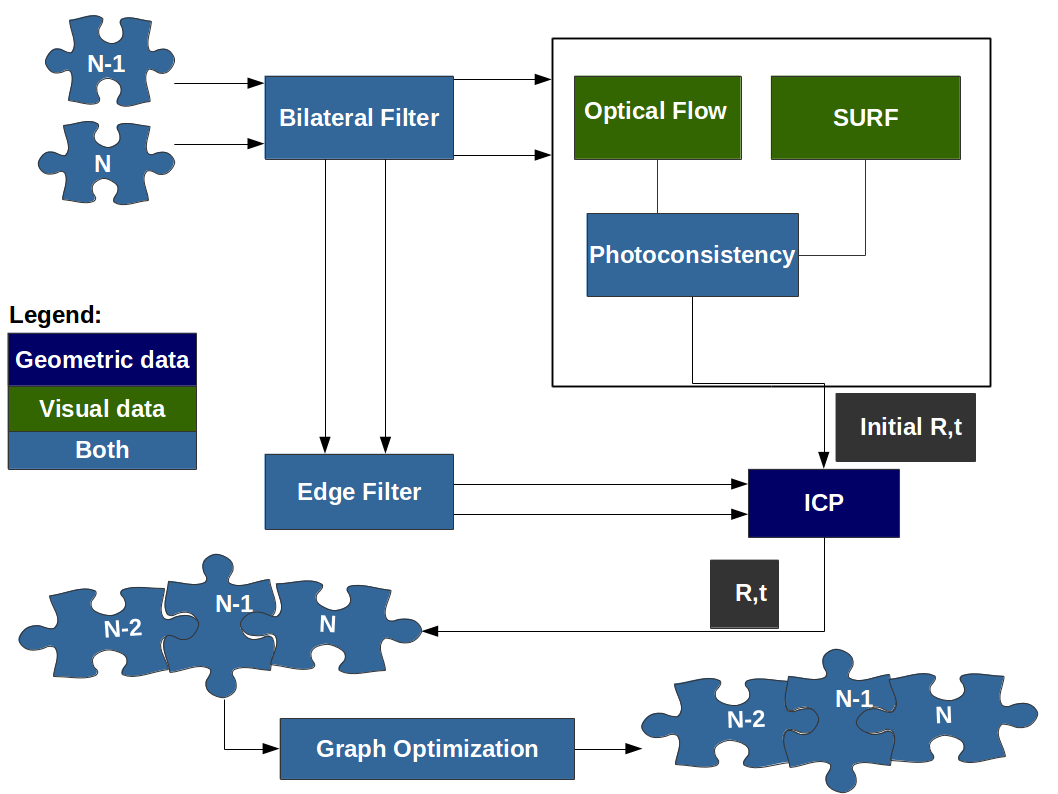
\includegraphics[scale=0.45]{images/complete_system}
\caption{Complete system}
\end{center}
\end{figure}

